\documentclass{article}

% Language setting
% Replace `english' with e.g. `spanish' to change the document language
\usepackage[english]{babel}

% Set page size and margins
% Replace `letterpaper' with `a4paper' for UK/EU standard size
\usepackage[letterpaper,top=2cm,bottom=2cm,left=3cm,right=3cm,marginparwidth=1.75cm]{geometry}
\usepackage{bm}

\usepackage[utf8]{inputenc} % 设置编码为UTF-8
\usepackage[T1]{fontenc}


% Useful packages
\usepackage{amsmath}
\usepackage{amssymb}

\usepackage{algorithm}
\usepackage{algpseudocode}

\usepackage{graphicx}
\usepackage{subfig}
\usepackage{float} 
\usepackage[colorlinks=true, allcolors=blue]{hyperref}
\usepackage{tikz}
\usepackage{palatino}
\usetikzlibrary{shapes.geometric, arrows}

% Costume Style Begin
\usepackage{enumitem}
% Costume Style End

% Operator Declaration Begin

% Operator Declaration End

\title{SUSTech CS303 2023 Fall Project2 Report}
\author{Chunhui XU}

\begin{document}
\maketitle

\section{Subtask 1}

\subsection{Introduction}

\subsubsection{Subtask 1 Introduction}
Different from the algorithm design of Project 1, Project 2 is an introductory attempt at a simple machine learning problem. Subtask 1 involves an image classification task. Under the training model provided by the \texttt{SoftmaxRegression} class, try to realize a simple image classification.

\subsubsection{Purpose}
Subtask 1 has already provided an encapsulated class, including internal code implementation and externally provided APIs, allowing us to briefly experience the machine learning process and understand some necessary parameter settings.

%% State the purpose of this subtask.


\subsection{Methodology}

\subsubsection{Algorithm/Model Design}
In Algorithm 1, I use pseudo-code to show the softmax regression training process provided by demo, including detailed algorithm details. In Algorithm 2, I used more abstract and simplified pseudo-code, hidden details but closer to the original idea of pseudo-code.


This "fit" process can be divided into these parts:
\begin{enumerate}
    \item \textbf{Compute logits and softmax probabilities}: The model first calculates the logits, which are the raw predictions that the model makes. The logits are then passed through the softmax function, which converts them into probabilities.
    \item \textbf{Compute loss}: The model then calculates the loss, which measures how far the model's predictions are from the true values. For Softmax Regression, we typically use the cross-entropy loss.
    \item \textbf{Update model parameters}: The model uses the gradients of the loss with respect to the model parameters to update the parameters. This is done using a method called gradient descent, which adjusts the parameters to minimize the loss.
    \item \textbf{Compute training accuracy}: The model calculates the accuracy on the training data to monitor the training process.
    \item If validation data is provided, the model also computes the logits, softmax probabilities, loss, and accuracy on the validation data. This allows us to monitor the model's performance on unseen data.
\end{enumerate}


\begin{algorithm}
\caption{Softmax Regression Training}
\begin{algorithmic}[1]

\Procedure{Fit}{$X\_train$, $y\_train$, $X\_val$, $y\_val$}
    \State $X\_train \gets$ add bias term to $X\_train$
    \State $trainLosses \gets$ empty list
    \State $valLosses \gets$ empty list
    \State $trainAccuracies \gets$ empty list
    \State $valAccuracies \gets$ empty list
    \For{$iteration \gets 1$ to $numIterations$}
        \State $logits \gets X\_train \cdot weights$
        \State $expLogits \gets e^{logits}$
        \State $softmaxProbs \gets expLogits /$ sum of $expLogits$ over samples
        \State $loss \gets -$ mean of $y\_train \cdot \log(softmaxProbs)$
        \State $gradient \gets (X\_train^T \cdot (softmaxProbs - y\_train)) /$ number of samples
        \State $weights \gets weights - learningRate \cdot gradient$
        \State $trainPred \gets$ argmax of $softmaxProbs$ over classes
        \State $trainAccuracy \gets$ mean of $(trainPred == y\_train)$
        \State Add $trainAccuracy$ to $trainAccuracies$
        \State Add $loss$ to $trainLosses$
        \If{$X\_val$, $y\_val$ is not None}
            \State $X\_val \gets$ add bias term to $X\_val$
            \State $logitsVal \gets X\_val \cdot weights$
            \State $expLogitsVal \gets e^{logitsVal}$
            \State $softmaxProbsVal \gets expLogitsVal /$ sum of $expLogitsVal$ over samples
            \State $valLoss \gets -$ mean of $y\_val \cdot \log(softmaxProbsVal)$
            \State $valPred \gets$ argmax of $softmaxProbsVal$ over classes
            \State $valAccuracy \gets$ mean of $(valPred == y\_val)$
            \State Add $valLoss$ to $valLosses$
            \State Add $valAccuracy$ to $valAccuracies$
        \EndIf
    \EndFor
    \State Output $trainLosses$, $valLosses$, $trainAccuracies$, $valAccuracies$
\EndProcedure
\end{algorithmic}
\end{algorithm}


\begin{algorithm}
\caption{Softmax Regression Training Abstract}
\begin{algorithmic}[1]
\Procedure{Initialize}{$num\_classes$, $learning\_rate$, $num\_iterations$}
    \State Initialize model parameters
\EndProcedure

\Procedure{Fit}{$X\_train$, $y\_train$, $X\_val$, $y\_val$}
    \For{$iteration \gets 1$ to $numIterations$}
        \State Compute logits and softmax probabilities for $X\_train$
        \State Compute loss using cross-entropy
        \State Update model parameters using gradient descent
        \State Compute training accuracy
        \If{validation data is provided}
            \State Compute logits and softmax probabilities for $X\_val$
            \State Compute validation loss using cross-entropy
            \State Compute validation accuracy
        \EndIf
    \EndFor
    \State \Return training and validation losses and accuracies
\EndProcedure
\end{algorithmic}
\end{algorithm}

\subsubsection{Analysis}

During training, the algorithm performs several operations for each iteration over the training dataset. Assume $n$ is the number of features in the dataset and $m$ is the number of examples in the training set, $k$ is the number of classes in the target variable..

\begin{itemize}
    \item For each example, the algorithm computes a linear combination of the input features and the weights. This step has a time complexity of O(n) for each example and class, resulting in a total of O(k*m*n) for the entire dataset.
    \item The softmax function is applied to the logits for each example to obtain probabilities.  This step is O(k) for each example since it needs to be computed for each class, so the total is O(k*m).
    \item Calculating the cross-entropy loss and gradients involves computing the loss for each example and then the gradient with respect to the weights. The gradient computation is O(k*n) per example. Hence, the total complexity for this step is O(k*m*n).
    \item At last, the weights are updated based on the gradients. The update step itself is O(n) because it involves updating each weight.
\end{itemize}

The overall time complexity is O(k*m*n) deciding part is calculating loss.


\subsection{Experiments}
\subsubsection{Metrics}
I use the argument \texttt{train\_accuracies} in \texttt{image\_classification\_demo.ipynb} to evaluate the accuracy improvement. Actually, for subtask 1 I changed the learning rate.

\subsubsection{Result}
The accuracy result of my submit is $0.5056516955086526$.

\subsubsection{Discovery}
I use four different learning rate to show the different feature.

\begin{figure*}[!ht]
    \centering
    \subfloat[learning rate=0.001]{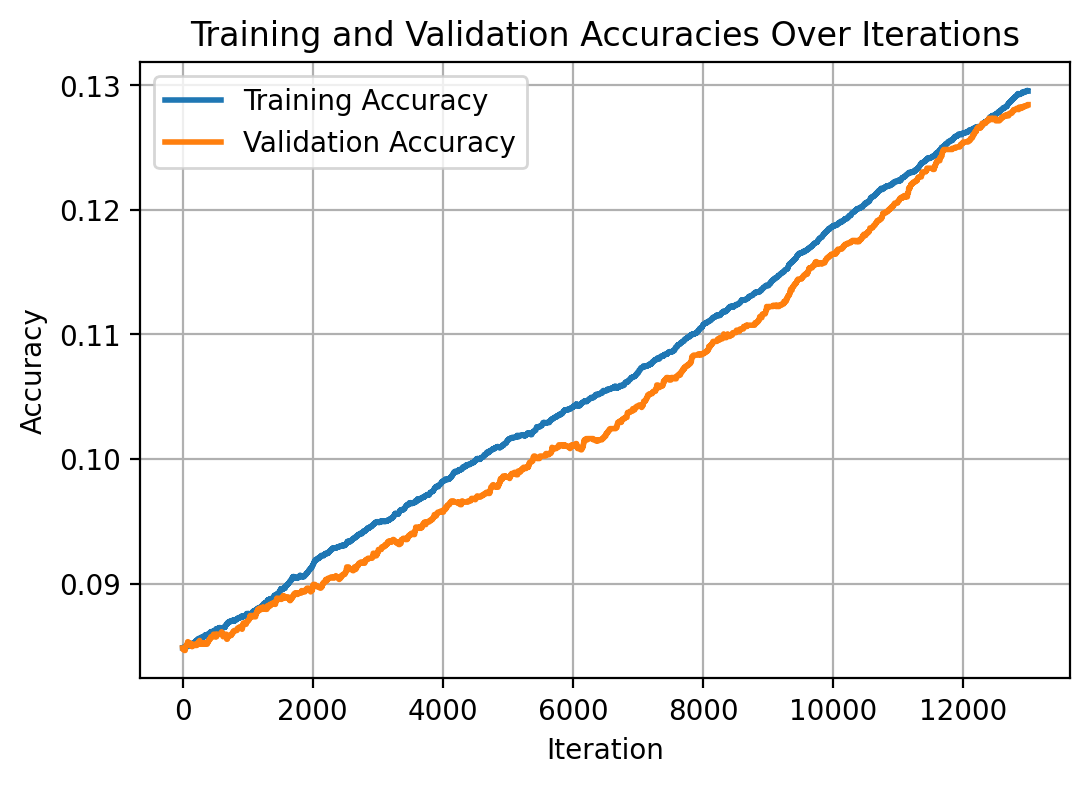
\includegraphics[width=0.45\textwidth]{img/sub1rate0.001.png}
    \label{r0.001a}}
    \hfill
    \subfloat[learning rate=0.01]{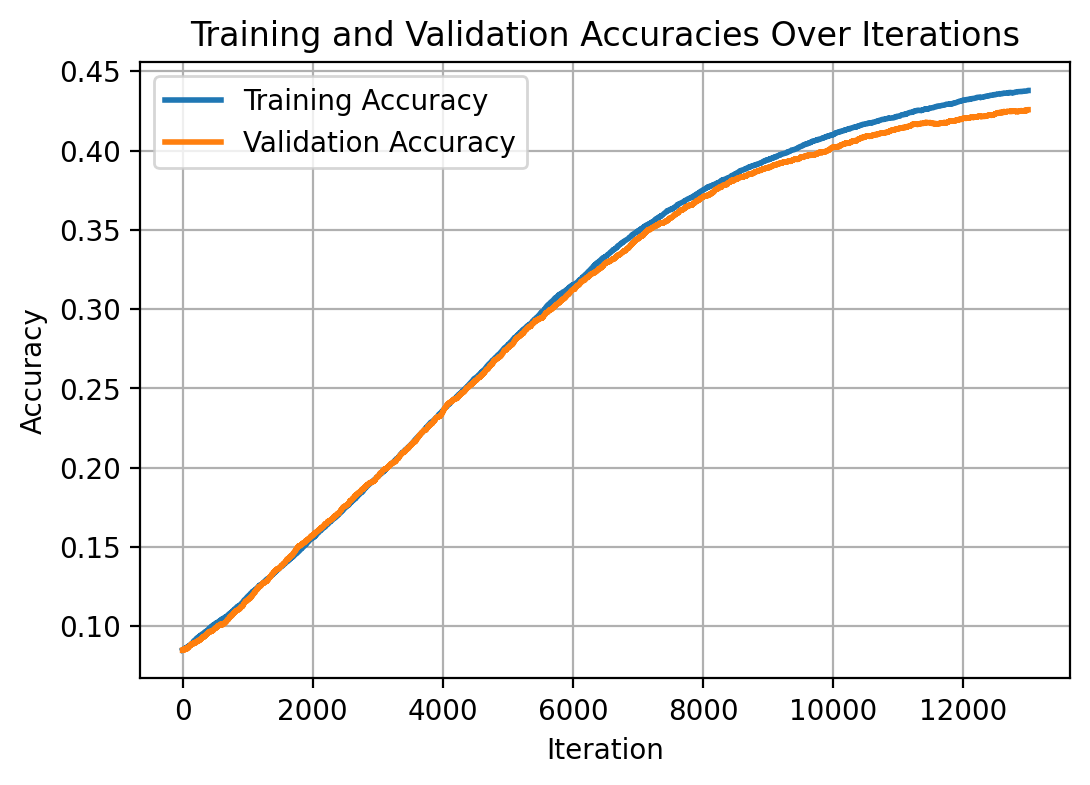
\includegraphics[width=0.45\textwidth]{img/sub1rate0.01.png}
    \label{r0.01a}}
    
    \subfloat[learning rate=0.05]{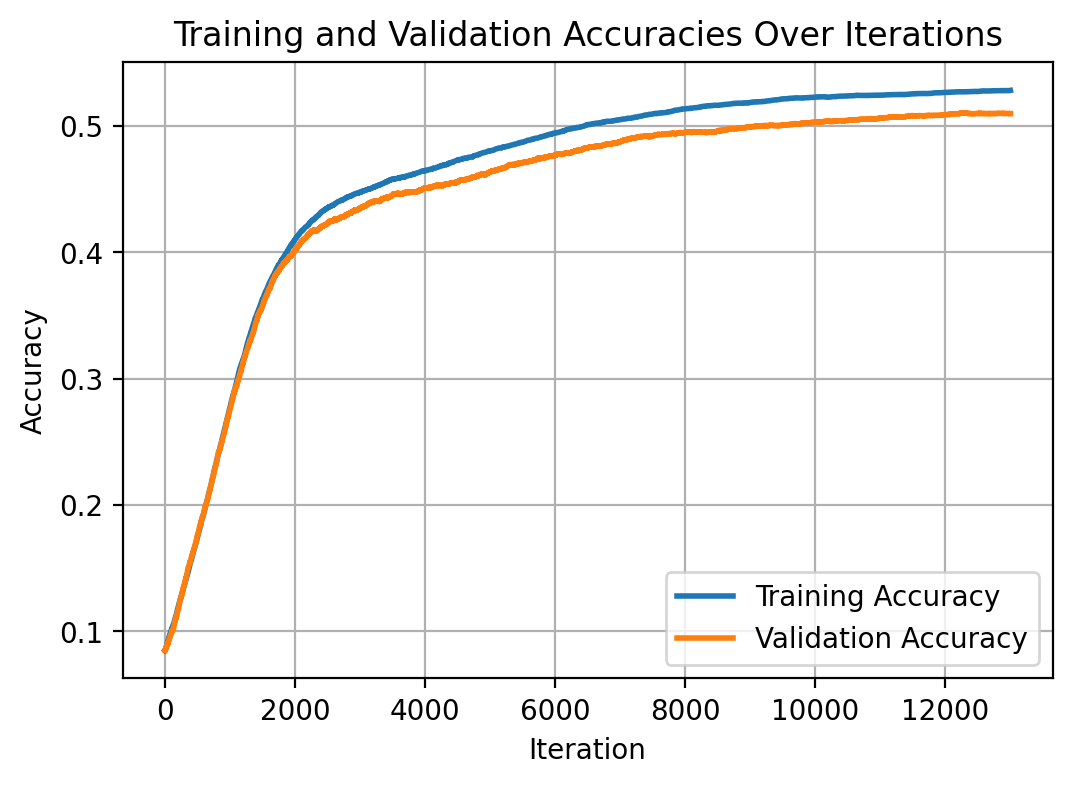
\includegraphics[width=0.45\textwidth]{img/sub1rate0.05.png}
    \label{r0.05a}}
    \hfill
    \subfloat[learning rate=0.2]{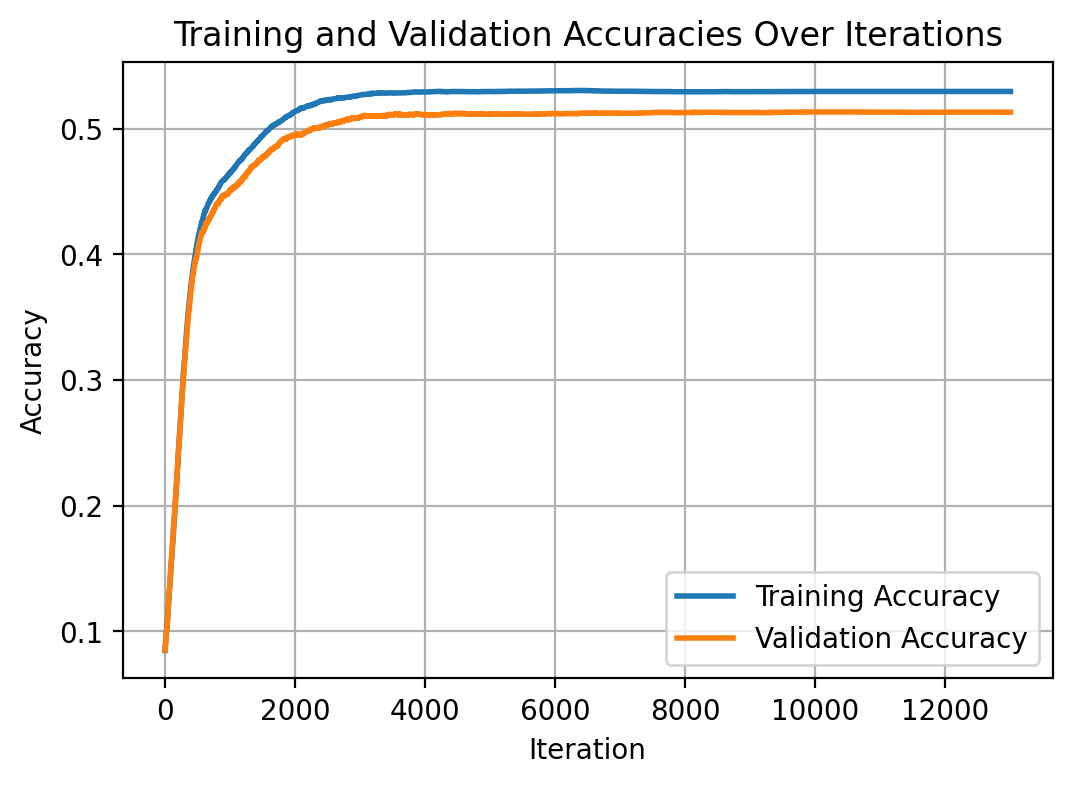
\includegraphics[width=0.45\textwidth]{img/sub1rate0.2.png} 
    \label{r0.2a}}
    \caption{Different learning rate accuracy in 12000 iterations}
    \label{fig:different_rate}
\end{figure*}

From Figure \ref{fig:different_rate}, We can see that: as the learning rate is smaller, the accuracy curve changes greatly, the overall accuracy is rising slowly. In other words, a smaller learning rate tends to make learning more accurate, and there is less possibility of missing the optimal solution.

As the learning rate becomes larger, the curve becomes steeper at beginning and smoother. But when the accuracy reaches the bottleneck, more iterations cannot bring better improvement to the model, because the higher learning rate means that the model loss the opportunity of smaller adjustments. This results in its accuracy bottleneck being lower.

However, given our limited number of iterations (limited personal PC performance), a high learning rate can bring the accuracy to climb faster, so the overall training efficiency can be greatly improved. But this is not suitable for model training with higher accuracy requirements.

\subsection{Further thoughts}

In this part, I know the simply realize of softmax regression model by demo. In fact, in image classification field, there are many different model. One of the most famous model is CNN. And this field has strong connection with computer vision.

If I have enough time, I will do a more in-depth comparison of features and efficiency between different models. I think this can lead me to a more complex field of machine learning.

\section{Subtask 2}

\subsection{Introduction}
\subsubsection{Background}
Nearest neighbor search is a common computer algorithm used to find the data point in a given data set that is most similar to a query point. Its goal is to find the nearest neighbors to a query point in order to perform various tasks such as classification, clustering, regression, etc. In image processing, nearest neighbor search is often used for image similarity measurement and image retrieval.

In image retrieval, nearest neighbor search is widely used to calculate the similarity between a query image and images in the database. Usually, the similarity between images is measured by calculating the distance or similarity measure between the image feature.

\subsubsection{Purpose}
The nearest neighbor search algorithm can then be used to find the image in the database that is most similar to the query image. One of the most commonly used nearest neighbor search algorithms is the k-nearest neighbor algorithm (k-NN), which finds the k neighbors most similar to a query point in a given data set. In image retrieval, the k-NN algorithm can be used to find the k images most similar to the query image, thereby achieving the goal of image retrieval.

Use NNS, we will try to find the 5 nearest image from the given image repository.

\begin{enumerate}
\item Give a general introduction to the subtask 2.
\item State the purpose of this subtask.
\end{enumerate}

\subsection{Methodology}
\subsubsection{Algorithm Design}

\begin{algorithm}
\caption{predict}
\begin{algorithmic}[1]
\Function{predict}{$x, X_{train}$}
    \State $distances \gets \sum_{i=1}^{n}((x - x_i)^2)^{0.4}, i \in X_{train}$
    \State \text{sort the distance}
    \State $k_{\text{indices}} \gets \text{the five smallest distance}$
    \State \textbf{return} $k_{\text{indices}}$
\EndFunction
\end{algorithmic}
\end{algorithm}

\subsubsection{Analyze}
Assume the retrieval repository data size is $n$, single data shape is $k$ (256 in this sub task). 

\begin{enumerate}
    \item For calculate single distance, we need time complexity O(k), calculate the whole distance will need: O($n*k$).
    \item Sort them: O($n \log n$). So single test data will be O($n*k + n \log n$). And this is the deciding part.
\end{enumerate}

\subsection{Experiments}
\subsubsection{Metrics}
In this subtask, I can only verify my result by sending it to online judge, so I have not found appropriate method to realize efficient comparisons and measurements.
\subsubsection{Result}
My accuracy for submit is $0.0506000000000001$

\subsubsection{Discovery}
I simply converted the Euclidean metric into a simple linear superposition and achieved a modest improvement in accuracy. My guess is that among the 256 features, there are some key features that can determine the similarity of two images, while other features are relatively insignificant.

However, in the Euclidean metric, if the difference between these irrelevant features is too large, they will also have a great impact on the image similarity measurement, so that two similar images will be judged as unrelated. 

Therefore, in actual image retrieval problems, we first need to find some features that have an important impact on image recognition accuracy during training, and then implement algorithms such as kNN based on these important features (that is, set appropriate weights is still very important) to prevent important feature differences from being ignored, or unimportant features being emphasized incorrectly.

\subsection{Further thoughts}
In fact, there are many more rigorous and efficient ways to implement kNN search. Moreover, in real problems, we can combine the kNN algorithm with many other optimizations.

For example, in subtask 3, we use mask to select features that can make the operation more accurate. If we want to apply mask in our image classification and retrieval algorithm, it means that we do not need to add all features to the distance calculation, but only need to select the feature with a mask value of 1, that is, the selected feature feature. In this case, we can reduce the k value and speed up the distance calculation.

Moreover, we can use more different algorithm to realize nearest neighbor search, such as Space partitioning, Locality-sensitive hashing and so on.

\section{Subtask 3}

\subsection{Introduction}

\subsubsection{Subtask 3 Introduction}
In the field of image classification, we may use masks to improve our recognition accuracy. For example, if the image in certain dataset always have a frame, the frame may be useless in classification. In that case, we want to ignore the frame feature by using mask.

In general, the role of mask code in image classification tasks is to help the model better understand and process target objects, thereby improving the accuracy and robustness of classification.

\subsubsection{Purpose}
This task gives us an opportunity to simulate the use of mask: use a simple 01 to represent the value of mask, and then use vector dot product to simulate the process of mask, allowing us to experience the role of mask and focus on the so-called ROI (Region of Interest).

\subsection{Methodology}
\subsubsection{Problem representation}
In this subtask, each data can be converted into 256 features. For these 256 features, we need to choose the appropriate mask and set the data at the 256 positions to 0 or 1, that is, only select some features as key data for predict. The selected features is the position which is 1 in mask. In this way, we can block out some features that are not helpful or even misleading for correct predictions.

\subsubsection{Algorithm/model design}

In this subtask, I try to generate the mask by random seed from 1 to 5000. Then run the \texttt{feature\_selection.ipynb} and \texttt{image\_recognition.ipynb} successively. Try to find a max accuracy of mask. I will describe its logic using a block diagram below:

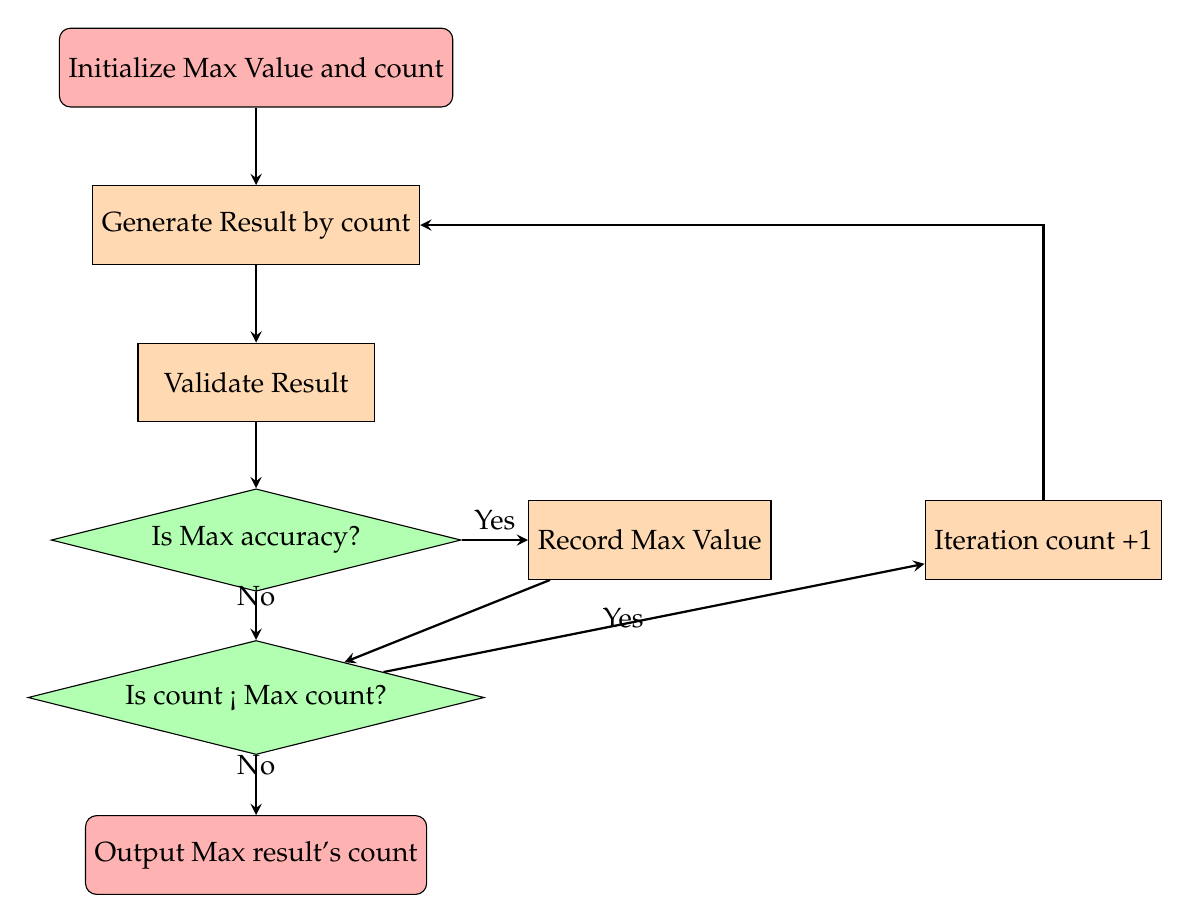
\begin{tikzpicture}[node distance=2cm]

\tikzstyle{startstop} = [rectangle, rounded corners, minimum width=3cm, minimum height=1cm,text centered, draw=black, fill=red!30]
\tikzstyle{process} = [rectangle, minimum width=3cm, minimum height=1cm, text centered, draw=black, fill=orange!30]
\tikzstyle{decision} = [diamond, draw, text badly centered,  aspect=4,fill=green!30]
\tikzstyle{arrow} = [thick,->,>=stealth]

\node (A) [startstop] {Initialize Max Value and count};
\node (B) [process, below of=A] {Generate Result by count};
\node (C) [process, below of=B] {Validate Result};
\node (D) [decision, below of=C] {Is Max accuracy?};
\node (G) [decision, below of=D] {Is count < Max count?};
\node (E) [process, right of=D, xshift=3cm] {Record Max Value};
\node (H) [process, right of=E, xshift=3cm] {Iteration count +1};
\node (I) [startstop, below of=G] {Output Max result's count};

\draw [arrow] (A) -- (B);
\draw [arrow] (B) -- (C);
\draw [arrow] (C) -- (D);
\draw [arrow] (D) -- node[anchor=south] {No} (G);
\draw [arrow] (D) -- node[anchor=south] {Yes} (E);
\draw [arrow] (E) -- (G);
\draw [arrow] (G) -- node[anchor=east] {Yes} (H);
\draw [arrow] (G) -- node[anchor=south] {No} (I);
\draw [arrow] (H) |- (B);

\end{tikzpicture}
\subsubsection{Analysis}
Consider $m$ is the max iteration count I have, $n$ is the shape of verify data. I do not consider the cost of train model, just verify the accuracy of the mask for original 10000 iterations for model train.

Generate mask code is O(1). Verify the data is O(n), the whole time complexity is O(mn).

\subsection{Experiments}
\subsubsection{Metrics}
The testing process has been explained in the above block diagram, that is, generating a mask and using the verification set to calculate its accuracy. Choose a random number seed between 1-5000 that maximizes accuracy.


\subsubsection{Result}
I found seed $1428$ for mask code can maximize the accuracy, which is $0.3092236894757903$


\subsection{Further thoughts}
I simply simulated using different random number seeds and selected a relatively best result in 5000 iterations. But this is only for smaller masks. When the shape of the mask increases, for example, there is a mask with a length of 10,000 waiting to be calculated, or when the dimension of the mask is larger, it is not enough to just use simple random generation.

I think the simulated annealing algorithm is suitable for this problem of finding a mask: for each mask, its local optimal solution can be found (which is usually a part of the global optimal solution in this problem), and iterations continue to obtain a mask solution of the highest accuracy.


\end{document}